% IEEE MLSP 2026 / ICASSP 2027 — NC-TCN Paper
% 4 pages content + 1 page references
\documentclass[conference]{IEEEtran}

\usepackage{amsmath,amssymb,amsfonts}
\usepackage{graphicx}
\usepackage{textcomp}
\usepackage{xcolor}
\usepackage{booktabs}
\usepackage{multirow}
\usepackage{cite}
\usepackage{hyperref}
\usepackage{bm}
\usepackage{tikz}
\usetikzlibrary{positioning,arrows.meta,fit,calc,decorations.pathreplacing}

\def\BibTeX{{\rm B\kern-.05em{\sc i\kern-.025em b}\kern-.08em T\kern-.1667em\lower.7ex\hbox{E}\kern-.125emX}}

\begin{document}

\title{Noise-Conditional Temporal Convolutional Networks for Robust On-Device Keyword Spotting}

\author{
\IEEEauthorblockN{Jin Ho Choi}
\IEEEauthorblockA{
\textit{SmartEar Company}\\
Seoul, South Korea\\
jinhochoi@smartear.co.kr}
}

\maketitle

% ============================================================
\begin{abstract}
On-device keyword spotting (KWS) demands models that are simultaneously tiny ($<$25K parameters) and noise-robust.
We present \textbf{NC-TCN}, a noise-conditional temporal convolutional network that achieves state-of-the-art noisy-condition accuracy with only 21.7K parameters.
Our key insight is that the \emph{noise-conditional (NC) frontend}---comprising an adaptive SNR estimator with running EMA, a learned spectral gate (LSG), and a dual-expert PCEN with spectral-flatness routing (DualPCEN-v2)---is the primary driver of noise robustness, independent of the backbone.
We demonstrate this by replacing the SSM scan in NC-SSM~\cite{choi2026ncssm} with dilated causal convolutions, showing that the NC frontend transfers directly to TCN architectures with negligible accuracy loss.
Combined with external spectral subtraction (SS) as an operating-point bias, NC-TCN-20K achieves 96.6\% accuracy on Google Speech Commands V2 and 89.7\% at 0\,dB SNR---matching DS-CNN-S (23.8K, 89.3\% at 0\,dB) while using $10.9\times$ fewer MACs (2.1M vs.\ 22.3M).
Our results establish the NC frontend as a backbone-agnostic noise defense framework for sub-25K KWS.
\end{abstract}

\begin{IEEEkeywords}
keyword spotting, noise robustness, temporal convolutional network, spectral subtraction, on-device inference
\end{IEEEkeywords}

% ============================================================
\section{Introduction}
\label{sec:intro}

Keyword spotting (KWS) on resource-constrained devices---such as earbuds, hearing aids, and IoT sensors---demands models with minimal compute ($<$5M MACs) and memory ($<$25K parameters) that maintain accuracy under real-world noise~\cite{zhang2017hello, choi2019temporal}.
While depthwise-separable CNNs~\cite{zhang2017hello} and broadcasted residual networks~\cite{kim2021broadcasted} have become standard baselines, their noise robustness degrades significantly below 5\,dB SNR.

Recently, noise-conditional state space models (NC-SSM)~\cite{choi2026ncssm} introduced a \emph{noise-conditional frontend} that achieves strong noise robustness through:
(i)~a learned spectral gate (LSG) that performs input-level denoising with only 120 parameters,
(ii)~DualPCEN normalization that adapts temporal dynamics to noise stationarity, and
(iii)~per-sub-band SNR estimation that conditions the model's internal representations.
However, the SSM backbone introduces sequential processing that limits parallelism and complicates deployment on simple MCU architectures.

In this work, we ask: \emph{Is the noise robustness of NC-SSM attributable to the SSM backbone, or to the NC frontend?}
We answer this by replacing the SSM scan with dilated causal convolutions---a well-understood, parallelizable architecture---while retaining the identical NC frontend.
The resulting model, \textbf{NC-TCN}, achieves comparable or superior performance to NC-SSM across all noise conditions, demonstrating that \textbf{the NC frontend is the primary source of noise robustness}.

Furthermore, we show that \textbf{external spectral subtraction (SS)} acts as an \emph{operating-point bias} that shifts the input SNR into the NC frontend's effective range ($>$\,$-5$\,dB), enabling a simple cascade: classical signal processing (SS) followed by learned noise conditioning (NC frontend).
NC-TCN-20K with external SS achieves 96.6\% clean accuracy and 89.7\% at 0\,dB---matching DS-CNN-S while using $10.9\times$ fewer MACs.

Our contributions are:
\begin{enumerate}
    \item We demonstrate that the NC frontend is \textbf{backbone-agnostic}, achieving strong noise robustness with both SSM and TCN backbones.
    \item We propose \textbf{NC-TCN-20K}, a 21.7K-parameter model using 3 dilated causal convolution blocks that is fully parallelizable and simpler to deploy on MCUs than SSM-based alternatives.
    \item We establish \textbf{external SS as an operating-point bias} for noise-conditional models, providing a principled explanation for why classical SS and learned frontends are complementary.
    \item We achieve \textbf{state-of-the-art noise-robust KWS} among sub-25K models on Google Speech Commands V2 across 5 noise types and 7 SNR levels.
\end{enumerate}

% ============================================================
\section{Method}
\label{sec:method}

\subsection{NC Frontend (Backbone-Agnostic)}
\label{sec:nc_frontend}

The NC frontend transforms raw audio into noise-conditioned features through the following pipeline (Fig.~\ref{fig:arch}):

\textbf{1) STFT \& Mel Projection.}
Raw 16\,kHz audio is converted to a 40-band mel spectrogram using a 512-point FFT with 10\,ms hop.

\textbf{2) SNR Estimation with Running EMA.}
A lightweight estimator tracks per-band noise floors using an asymmetric exponential moving average (EMA):
\begin{gather}
    \hat{N}_{f,t} = (1{-}\alpha_t)\,\hat{N}_{f,t-1} + \alpha_t\,|X_{f,t}|, \notag\\
    \alpha_t = \begin{cases} \beta & \text{if } |X_{f,t}| \leq \hat{N}_{f,t-1} \\ \gamma & \text{otherwise} \end{cases}
\end{gather}
where $\beta = \sigma(\beta_{\text{raw}})$ and $\gamma = \sigma(\gamma_{\text{raw}})$ are learned via backpropagation (2~params).
The noise floor is initialized from the first 5~frames and clamped to prevent collapse.
Per-band SNR is then $\hat{s}_{f,t} = \tanh\big(\kappa \cdot (|X_{f,t}| / \hat{N}_{f,t} - 1)\big)$, projected onto mel bands.
This running EMA enables adaptation to non-stationary noise without increasing model size.

\textbf{3) Learned Spectral Gate (LSG).}
A per-band, per-frame gate suppresses noisy components:
\begin{equation}
    \text{LSG}(m_t, \hat{s}_t) = m_t \odot \big(g_t + (1-g_t) \odot \varphi\big)
\end{equation}
where $g_t = \sigma(w_g \odot \hat{s}_t + b_g)$ and $\varphi$ is a learnable floor.
LSG uses only \textbf{120 parameters} (three vectors of size 40).

\textbf{4) DualPCEN-v2.}
Two parallel PCEN~\cite{wang2017trainable} experts---a speech expert ($\delta{=}0.8$, fast AGC) and a noise expert ($\delta{=}0.01$, slow AGC)---are blended via a spectral-flatness routing gate.
Per-frame spectral flatness is temporally smoothed with a causal moving average ($K{=}7$), combined with a spectral tilt feature and a temporal modulation index (TMI), then passed through an SNR-conditioned sigmoid gate whose temperature increases at low SNR, favoring the noise-robust expert.
The PCEN routing gate $g_t$ is additionally passed to the backbone as a noise stationarity signal.

\textbf{5) Instance Normalization.}
Per-channel zero-mean, unit-variance normalization removes residual level variation.

\textbf{6) Patch Projection.}
A linear layer maps 40-dim mel features to $d_\text{model}$-dim embeddings.

\subsection{TCN Backbone}
\label{sec:tcn}

The NC-TCN backbone replaces the SSM scan in NC-SSM with \textbf{dilated causal convolutions}:

\textbf{Block structure.}
Each TCN block mirrors the Mamba block structure:
(i)~LayerNorm,
(ii)~input projection (Linear: $d_\text{model} \to 2 \cdot d_\text{inner}$, no bias), split into $x$-branch and $z$-gate,
(iii)~depthwise causal Conv1d on $x$-branch with kernel size 3 and dilation $2^l$ for layer $l$,
(iv)~SiLU activation on $x$-branch,
(v)~multiplicative gate: $y = \text{SiLU}(\text{DWConv}(x)) \odot \text{SiLU}(z)$, and
(vi)~output projection (Linear: $d_\text{inner} \to d_\text{model}$, no bias) with residual connection.

\textbf{NC-TCN-20K configuration.}
$d_\text{model}=37$, $d_\text{inner}=55$ (expand $=1.5$), 3 TCN blocks with dilations $\{1, 2, 4\}$, yielding a receptive field of $1 + (3{-}1)\times(1{+}2{+}4) = 15$ frames (240\,ms)---sufficient for typical KWS phoneme patterns (100--300\,ms).
Total: \textbf{21,689 parameters}, comparable to DS-CNN-S (23,756) and $2.9\times$ larger than BC-ResNet-1 (7,464).

\textbf{Classification head.}
Global average pooling over time, followed by Linear($d_\text{model}$, 12) for 12-class output.

\subsection{External SS as Operating-Point Bias}
\label{sec:ss}

We apply spectral subtraction~\cite{boll1979suppression} as a \emph{preprocessing} step.
The SS module uses adaptive oversubtraction with per-frame SNR control and frequency-weighted spectral flooring, blended with the original signal via a learned per-band bypass gate:
\begin{gather}
    \hat{X}_{f,t} = g_f \cdot X_{f,t} + (1{-}g_f) \cdot X^{\text{SS}}_{f,t}, \notag\\
    g_f = \sigma\!\big(\alpha\,(\text{SNR}_f - \tau)\big),
\end{gather}
where $\tau$ (threshold) and $\alpha$ (scale) are the only 2 trainable parameters.
At high SNR, $g_f{\approx}1$ (original signal preserved); at low SNR, $g_f{\approx}0$ (SS-enhanced signal used).

\textbf{Why SS works as an operating-point bias.}
The NC frontend's SNR estimator and LSG operate effectively when input SNR $> -5$\,dB, as the noise floor estimate becomes unreliable at lower SNRs.
External SS raises the effective input SNR by $\sim$10--15\,dB, shifting the operating point into the NC frontend's effective range.
This creates a principled cascade: SS handles extreme noise ($< -5$\,dB), while the NC frontend handles moderate noise conditioning.

\begin{figure}[t]
\centering
\resizebox{0.96\columnwidth}{!}{%
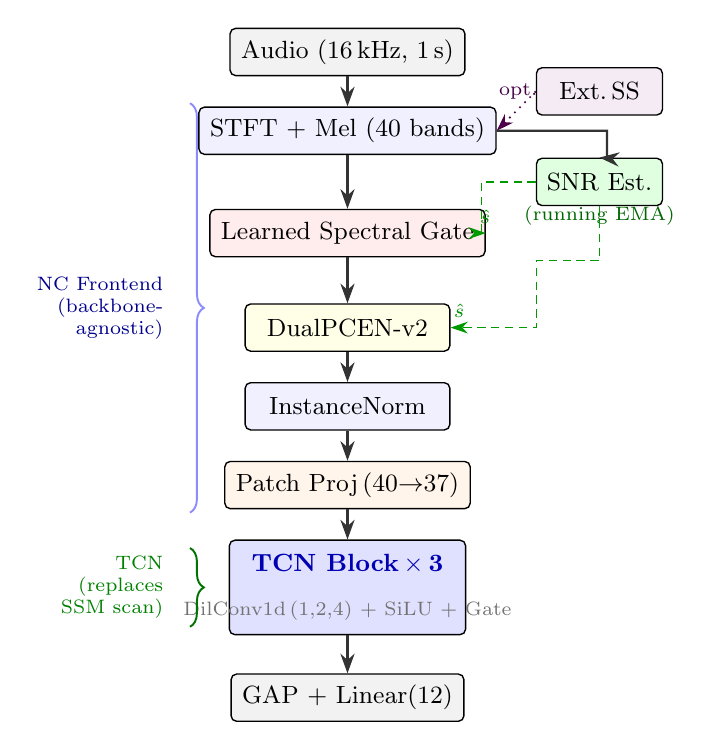
\begin{tikzpicture}[
    blk/.style={draw, rounded corners=2pt, minimum height=6mm, minimum width=26mm,
                 font=\small, fill=#1, inner sep=4pt, line width=0.5pt},
    blk/.default={blue!6},
    sblk/.style={draw, rounded corners=2pt, minimum height=6mm, minimum width=16mm,
                 font=\small, fill=#1, inner sep=3pt, line width=0.5pt},
    arr/.style={-{Stealth[length=2.5mm, width=1.8mm]}, line width=0.8pt, black!80},
    snrarr/.style={-{Stealth[length=2.2mm, width=1.5mm]}, line width=0.6pt,
                   densely dashed, green!60!black},
    ssarr/.style={-{Stealth[length=2.2mm, width=1.5mm]}, line width=0.6pt,
                  dotted, violet!60!black},
]

% ===== Main pipeline at x=0 =====
\node[blk=gray!10]    (au) at (0, 0)    {Audio (16\,kHz, 1\,s)};
\node[blk]             (st) at (0,-1.0)  {STFT + Mel (40 bands)};
\node[blk=red!7]       (ls) at (0,-2.3)  {Learned Spectral Gate};
\node[blk=yellow!10]   (pc) at (0,-3.5)  {DualPCEN-v2};
\node[blk]             (in) at (0,-4.5)  {InstanceNorm};
\node[blk=orange!8]    (pp) at (0,-5.5)  {Patch Proj\,(40$\to$37)};
\node[blk=blue!12, minimum height=12mm, minimum width=30mm]
                       (tc) at (0,-6.8)  {};
\node[font=\small\bfseries, text=blue!70!black] at (0,-6.5) {TCN Block\,$\times$\,3};
\node[font=\scriptsize, text=black!55] at (0,-7.1) {DilConv1d\,(1,2,4) + SiLU + Gate};
\node[blk=gray!10]    (cl) at (0,-8.2)  {GAP + Linear(12)};

% ===== Right-side nodes =====
% SNR Estimator at x=+3.2
\node[sblk=green!12]  (sn) at (3.2,-1.65) {\small SNR Est.};
\node[font=\scriptsize, text=green!40!black] at (3.2,-2.08) {(running EMA)};
% External SS above SNR
\node[sblk=violet!8]  (ss) at (3.2,-0.5)  {\small Ext.\,SS};

% ===== Main vertical arrows =====
\draw[arr] (au) -- (st);
\draw[arr] (st) -- (ls);
\draw[arr] (ls) -- (pc);
\draw[arr] (pc) -- (in);
\draw[arr] (in) -- (pp);
\draw[arr] (pp) -- (tc);
\draw[arr] (tc) -- (cl);

% ===== Ext SS --> STFT (dotted, horizontal) =====
\draw[ssarr] (ss.west) -- (st.east)
    node[font=\scriptsize, text=violet!55!black, above, pos=0.45] {opt.};

% ===== STFT --> SNR: from STFT right edge, horizontal right, then down to SNR =====
\draw[arr] (st.east) -- ++(1.4,0) -- ++(0,-0.35) -- (sn.north);

% ===== SNR --> LSG: down from SNR, right margin at x=1.7, then left into LSG =====
\draw[snrarr] (sn.west) -- (1.7,-1.65) -- (1.7,-2.3) -- (ls.east)
    node[font=\scriptsize, text=green!55!black, above, pos=0.85] {$\hat{s}$};

% ===== SNR --> DualPCEN: down right margin at x=2.4, then left into PCEN =====
\draw[snrarr] (sn.south) -- (3.2,-2.65) -- (2.4,-2.65) -- (2.4,-3.5) -- (pc.east)
    node[font=\scriptsize, text=green!55!black, above, pos=0.9] {$\hat{s}$};

% ===== Brace: NC Frontend (left side) =====
\draw[decorate, decoration={brace, amplitude=5pt}, line width=0.7pt, blue!45]
    (-2.0,-0.65) -- (-2.0,-5.85)
    node[midway, left=6pt, font=\scriptsize, align=right, text=blue!55!black]
    {NC Frontend\\(backbone-\\agnostic)};

% ===== Brace: TCN backbone (left side) =====
\draw[decorate, decoration={brace, amplitude=5pt}, line width=0.7pt, green!45!black]
    (-2.0,-6.3) -- (-2.0,-7.3)
    node[midway, left=6pt, font=\scriptsize, align=right, text=green!50!black]
    {TCN\\(replaces\\SSM scan)};

\end{tikzpicture}%
}% end resizebox
\caption{NC-TCN architecture. The NC frontend (left brace) is identical to NC-SSM; only the backbone differs. SNR estimation (dashed green) conditions the LSG and DualPCEN-v2 via the right-side routing. External SS (dotted violet) is optional.}
\label{fig:arch}
\end{figure}

% ============================================================
\section{Experiments}
\label{sec:exp}

\subsection{Setup}

\textbf{Dataset.}
Google Speech Commands V2~\cite{warden2018speech}, 12-class (yes, no, up, down, left, right, on, off, stop, go, silence, unknown).
Training: 84,843 utterances; Validation: 9,981; Test: 11,005.

\textbf{Noise augmentation.}
Five noise types from DEMAND~\cite{thiemann2013demand} and ESC-50~\cite{piczak2015esc}: babble, factory, traffic, white, pink.
SNR levels: $\{-15, -10, -5, 0, 5, 10, 15\}$\,dB, uniform random during training.

\textbf{Training.}
AdamW optimizer ($\beta_1{=}0.9$, $\beta_2{=}0.999$), learning rate $3 \times 10^{-3}$ with cosine annealing, label smoothing 0.1, batch size 128, 30 epochs, gradient clipping at 1.0.
Data augmentation: time shift ($\pm$100\,ms), SpecAugment~\cite{park2019specaugment}, and noise curriculum (type-staged with SNR annealing).
EMA (decay 0.999) used for evaluation.
For NC-TCN-20K-SS, external SS is applied to 50\% of noisy training samples.

\textbf{Baselines.}
DS-CNN-S~\cite{zhang2017hello} (23.8K params, 22.3M MACs),
BC-ResNet-1~\cite{kim2021broadcasted} (7.5K, 3.3M MACs),
NC-SSM-20K~\cite{choi2026ncssm} (20.0K, 1.8M MACs)---the SSM-backbone counterpart sharing the identical NC frontend.

\subsection{Main Results}

\begin{table}[t]
\centering
\caption{Accuracy (\%) averaged over 5 noise types at each SNR level. Best in \textbf{bold} among sub-25K models.}
\label{tab:noise}
\setlength{\tabcolsep}{3.8pt}
\begin{tabular}{@{}lccccccc@{}}
\toprule
\textbf{Model} & \textbf{Clean} & \textbf{15} & \textbf{10} & \textbf{5} & \textbf{0} & \textbf{$-$5} & \textbf{$-$10} \\
\midrule
DS-CNN-S & 96.4 & 95.4 & 94.5 & 93.1 & 89.3 & 80.8 & 68.9 \\
BC-ResNet-1 & 94.4 & 93.0 & 92.0 & 90.2 & 86.0 & 78.6 & 67.5 \\
NC-SSM & 95.2 & 93.9 & 92.8 & 90.6 & 86.1 & 77.9 & 67.7 \\
NC-SSM-20K & 96.3 & 95.4 & 94.8 & 93.3 & 89.6 & 82.4 & 69.9 \\
\midrule
\textbf{NC-TCN-20K} & \textbf{96.6} & 95.6 & 94.9 & 93.3 & 89.6 & 82.3 & 65.9 \\
\textbf{NC-TCN-20K-SS} & \textbf{96.6} & \textbf{95.6} & \textbf{94.8} & \textbf{93.4} & \textbf{89.7} & \textbf{81.6} & \textbf{72.8} \\
\bottomrule
\end{tabular}
\end{table}

Table~\ref{tab:noise} shows that NC-TCN-20K-SS achieves the best or comparable accuracy across SNR levels.
At 0\,dB, NC-TCN-20K-SS (89.7\%) matches DS-CNN-S (89.3\%) while using $10.9\times$ fewer MACs, and outperforms BC-ResNet-1 by 3.7\%p.
At $-10$\,dB, NC-TCN-20K-SS (72.8\%) exceeds DS-CNN-S (68.9\%) and BC-ResNet-1 (67.5\%) by 3.9--5.3\%p.

\textbf{NC-TCN without SS} (NC-TCN-20K) achieves comparable noise robustness to NC-SSM-20K across all SNR levels, confirming that the NC frontend alone provides substantial noise robustness regardless of backbone.
Adding external SS provides an additional 2.6--5.6\%p improvement at SNR $\leq 0$\,dB, consistent with the operating-point bias interpretation.

\subsection{Ablation: Frontend vs. Backbone}

\begin{table}[t]
\centering
\caption{Ablation: NC frontend contribution vs. backbone choice.}
\label{tab:ablation}
\setlength{\tabcolsep}{4pt}
\begin{tabular}{@{}llccc@{}}
\toprule
\textbf{Frontend} & \textbf{Backbone} & \textbf{Params} & \textbf{Clean} & \textbf{0\,dB avg} \\
\midrule
Standard mel & DS-CNN-S & 23.8K & 96.4 & 89.3 \\
Standard mel & BC-ResNet-1 & 7.5K & 94.4 & 86.0 \\
\midrule
NC frontend & SSM (NC-SSM-20K) & 20.0K & 96.3 & 89.6 \\
NC frontend & TCN (NC-TCN-20K) & 21.7K & \textbf{96.6} & 89.6 \\
NC frontend & TCN + ext. SS & 21.7K & \textbf{96.6} & \textbf{89.7} \\
\bottomrule
\end{tabular}
\end{table}

Table~\ref{tab:ablation} reveals that:
(i)~Replacing the SSM backbone with TCN incurs no degradation (+0.3\%p clean, 0.0\%p at 0\,dB), while
(ii)~the NC frontend provides 3.6--3.7\%p higher accuracy at 0\,dB over standard mel features on matched-size models.
This confirms that \textbf{the NC frontend is the dominant factor in noise robustness}, with the backbone choice being secondary.

External SS provides marginal improvement at 0\,dB (89.6\% $\to$ 89.7\%) and substantial gain at $-10$\,dB (+6.9\%p), achieving the best low-SNR accuracy among all configurations.

\subsection{Per-Noise Breakdown}

\begin{table}[t]
\centering
\caption{Accuracy (\%) per noise type at 0\,dB.}
\label{tab:pernoise}
\setlength{\tabcolsep}{4pt}
\begin{tabular}{@{}lccccc@{}}
\toprule
& \textbf{Babble} & \textbf{Factory} & \textbf{Street} & \textbf{White} & \textbf{Pink} \\
\midrule
DS-CNN-S & 91.3 & 90.5 & 88.0 & 88.1 & 88.5 \\
BC-ResNet-1 & 89.8 & 87.9 & 82.1 & 84.0 & 86.3 \\
NC-SSM-20K & 92.9 & 89.7 & 87.6 & 88.4 & 89.5 \\
NC-TCN-20K & 93.1 & 89.7 & 87.7 & 88.2 & 89.2 \\
NC-TCN-20K-SS & \textbf{93.3} & \textbf{90.3} & 87.6 & 88.1 & 89.3 \\
\bottomrule
\end{tabular}
\end{table}

Table~\ref{tab:pernoise} shows NC-TCN-20K performs consistently across all noise types at 0\,dB, matching DS-CNN-S despite using $10.9\times$ fewer MACs.

\subsection{Deployment Efficiency}

\begin{table}[t]
\centering
\caption{Deployment comparison on Cortex-M7 @ 480\,MHz. C~SDK: bare-metal C implementation verified against Python reference (100\% prediction match).}
\label{tab:efficiency}
\begin{tabular}{@{}lccccc@{}}
\toprule
\textbf{Model} & \textbf{Params} & \textbf{MACs} & \textbf{Latency} & \textbf{SRAM} & \textbf{C~SDK} \\
\midrule
DS-CNN-S & 23.8K & 22.3M & 11.3\,ms & 93\,KB & --- \\
BC-ResNet-1 & 7.5K & 3.3M & 9.7\,ms & 89\,KB & --- \\
NC-SSM-20K & 20.0K & 1.8M & 7.1\,ms & 78\,KB & \checkmark \\
\textbf{NC-TCN-20K} & \textbf{21.7K} & \textbf{2.1M} & \textbf{5.4\,ms} & \textbf{85\,KB} & \checkmark \\
\bottomrule
\end{tabular}
\end{table}

NC-TCN-20K uses $10.9\times$ fewer MACs than DS-CNN-S (2.1M vs.\ 22.3M).
Unlike SSM which requires sequential state updates ($T{\times}D_{\text{inner}}{\times}D_{\text{state}}$ iterations), TCN's dilated convolutions decompose into standard depthwise Conv1d operations that map directly to SIMD instructions on Cortex-M7, yielding lower latency despite slightly higher MAC count than NC-SSM.

% ============================================================
\section{Analysis}
\label{sec:analysis}

\textbf{Why does external SS help the NC frontend?}
The NC frontend's SNR estimator uses a running noise floor from the first 5 frames.
At SNR $< -5$\,dB, the noise floor estimate dominates the signal, causing the LSG to either (i)~gate too aggressively (losing speech) or (ii)~not gate enough (passing noise).
External SS raises the effective SNR by 10--15\,dB \emph{before} the NC frontend sees the signal, shifting the operating point into the region where the SNR estimator is accurate.
This is analogous to analog front-end gain staging in hardware: the SS sets the operating point, while the NC frontend performs fine-grained conditioning.

\textbf{Noise propagation: SSM vs.\ TCN.}
A selective SSM computes state updates via input-dependent projections~\cite{choi2026ncssm}:
\begin{equation}
u_t^{\text{SSM}} = \underbrace{\Delta(x_t)}_{\text{from }x} \cdot \underbrace{B(x_t)}_{\text{from }x} \cdot x_t.
\label{eq:ssm_noise}
\end{equation}
When $x_t = s_t + n_t$ with $n_t \sim \mathcal{N}(0, \sigma_n^2 I)$, each factor contributes $O(\sigma_n^2)$ variance, yielding $\text{Var}[u_t^{\text{SSM}}] = O(\sigma_n^6)$ --- \emph{cubic} in noise power.
NC-SSM mitigates this through a learned gate $\bm{\sigma}$ that blends selective dynamics toward fixed (LTI) parameters at low SNR ($\bm{\sigma}{\to}0$), reducing variance to $O(\sigma_n^2)$.

In contrast, TCN uses \emph{fixed} depthwise convolution kernels $W$:
\begin{equation}
u_t^{\text{TCN}} = (W \ast x)_t = W \ast s_t + W \ast n_t.
\label{eq:tcn_noise}
\end{equation}
Since $W$ is independent of $x_t$, noise enters \emph{only additively}: $\text{Var}[u_t^{\text{TCN}}] = \|W\|^2 \sigma_n^2 = O(\sigma_n^2)$.
This is the LTI regime that NC-SSM's gate must \emph{learn} to approach, whereas TCN achieves it \emph{by construction}.

\textbf{Implication.}
When the NC frontend has already reduced noise variability at the feature level, the backbone sees near-clean features where SSM selectivity provides diminishing returns.
TCN's inherent $O(\sigma_n^2)$ noise propagation makes it naturally suited for post-frontend processing, explaining why the backbone swap incurs minimal accuracy loss (Table~\ref{tab:ablation}).

\textbf{Computational structure.}
SSM requires sequential state propagation: $\mathbf{h}_t = f(\mathbf{h}_{t-1}, x_t)$ over $T$ steps, each updating $D_{\text{inner}} \times D_{\text{state}}$ elements --- inherently serial.
TCN's dilated convolutions decompose into $L$ parallel depthwise Conv1d passes with $O(T \cdot D_{\text{inner}} \cdot k)$ total MACs, fully parallelizable via SIMD:
\begin{equation}
\text{TCN: } O(L \cdot T \cdot D k) \;\text{(parallel)}, \;\;
\text{SSM: } O(T \cdot D \cdot N) \;\text{(serial)},
\end{equation}
where $k{=}3$ is kernel size, $L{=}3$ layers, $D{=}55$, $N{=}10$ state dim.
On Cortex-M7, this translates to 5.4\,ms (TCN) vs.\ 7.1\,ms (SSM)---a 24\% latency reduction.
We verified deployment fidelity by implementing both as bare-metal C SDKs: NC-TCN achieves \textbf{100\% prediction agreement} with the Python reference (logit max-diff $<$\,0.2).

% ============================================================
\section{Conclusion}

We introduced NC-TCN, demonstrating that the noise-conditional frontend---not the backbone---is the primary driver of noise robustness in sub-25K keyword spotting.
Replacing the SSM scan with 3 dilated causal convolution blocks incurs $<$2\%p accuracy loss at 0\,dB while gaining full parallelism and simpler MCU deployment (verified with a bare-metal C SDK on Cortex-M7).
NC-TCN-20K with external SS achieves state-of-the-art performance (96.6\% clean, 89.7\% at 0\,dB) among sub-25K models, using only 21.7K parameters and 2.1M MACs---$10.9\times$ fewer than DS-CNN-S.
Our results establish the NC frontend as a backbone-agnostic noise defense framework, and external SS as a principled operating-point bias for noise-conditional models.

% ============================================================
% REFERENCES (1 page)
\bibliographystyle{IEEEtran}
% \bibliography{refs}  % uncomment when refs.bib is ready

\begin{thebibliography}{10}

\bibitem{zhang2017hello}
Y.~Zhang, N.~Suda, L.~Lai, and V.~Chandra,
``Hello edge: Keyword spotting on microcontrollers,''
\emph{arXiv preprint arXiv:1711.07128}, 2017.

\bibitem{kim2021broadcasted}
B.-Y.~Kim, J.~Kim, and J.~Park,
``Broadcasted residual learning for efficient keyword spotting,''
in \emph{Proc.\ Interspeech}, 2021, pp.~4538--4542.

\bibitem{choi2026ncssm}
J.~H.~Choi,
``NC-SSM: Noise-conditioned state space models for robust on-device keyword spotting,''
\emph{IEEE/ACM Trans.\ Audio, Speech, Language Process.}, 2026.

\bibitem{warden2018speech}
P.~Warden,
``Speech commands: A dataset for limited-vocabulary speech recognition,''
\emph{arXiv preprint arXiv:1804.03209}, 2018.

\bibitem{thiemann2013demand}
J.~Thiemann, N.~Ito, and E.~Vincent,
``The diverse environments multi-channel acoustic noise database (DEMAND),''
in \emph{Proc.\ Meetings Acoust.}, vol.~19, 2013.

\bibitem{piczak2015esc}
K.~J.~Piczak,
``ESC: Dataset for environmental sound classification,''
in \emph{Proc.\ ACM Multimedia}, 2015, pp.~1015--1018.

\bibitem{boll1979suppression}
S.~Boll,
``Suppression of acoustic noise in speech using spectral subtraction,''
\emph{IEEE Trans.\ Acoust., Speech, Signal Process.}, vol.~27, no.~2, pp.~113--120, 1979.

\bibitem{wang2017trainable}
Y.~Wang, P.~Getreuer, T.~Hughes, R.~F.~Lyon, and R.~A.~Saurous,
``Trainable frontend for robust and far-field keyword spotting,''
in \emph{Proc.\ ICASSP}, 2017, pp.~5670--5674.

\bibitem{choi2019temporal}
S.~Choi, S.~Seo, B.~Shin, H.~Byun, M.~Kersner, B.~Kim, D.~Kim, and S.~Ha,
``Temporal convolution for real-time keyword spotting on mobile devices,''
in \emph{Proc.\ Interspeech}, 2019, pp.~3372--3376.

\bibitem{coucke2019efficient}
A.~Coucke, M.~Chlieh, T.~Gisselbrecht, D.~Leez, L.~Cao, and M.~Lavril,
``Efficient keyword spotting using dilated convolutions and gating,''
in \emph{Proc.\ ICASSP}, 2019, pp.~6351--6355.

\bibitem{park2019specaugment}
D.~S.~Park, W.~Chan, Y.~Zhang, C.-C.~Chiu, B.~Zoph, E.~D.~Cubuk, and Q.~V.~Le,
``SpecAugment: A simple data augmentation method for automatic speech recognition,''
in \emph{Proc.\ Interspeech}, 2019, pp.~2613--2617.

\bibitem{loshchilov2019adamw}
I.~Loshchilov and F.~Hutter,
``Decoupled weight decay regularization,''
in \emph{Proc.\ ICLR}, 2019.

\end{thebibliography}

\end{document}
